\documentclass[12pt,article,oneside]{memoir}
\usepackage{fontspec}
\usepackage{xunicode}
\usepackage{url}
\usepackage{rotating}
\usepackage{placeins}
\usepackage{tabu}
\usepackage{colortbl}
\usepackage{pdflscape}
\usepackage{memoir-article-styles}
\usepackage[american, british, norsk]{babel}
\usepackage[babel]{csquotes}
\usepackage[svgnames]{xcolor}
\usepackage{soul}
\usepackage[xetex, colorlinks=true, urlcolor=DarkSlateBlue,
citecolor=DarkSlateBlue, filecolor=DarkSlateBlue, plainpages=false,
pdfpagelabels, bookmarksnumbered]{hyperref}
\usepackage{etoolbox}

%% Pagestyle
\pagestyle{kjh}




\usepackage{color}
\usepackage{fancyvrb}
\newcommand{\VerbBar}{|}
\newcommand{\VERB}{\Verb[commandchars=\\\{\}]}
\DefineVerbatimEnvironment{Highlighting}{Verbatim}{commandchars=\\\{\}}
% Add ',fontsize=\small' for more characters per line
\newenvironment{Shaded}{}{}
\newcommand{\KeywordTok}[1]{\textcolor[rgb]{0.00,0.44,0.13}{\textbf{#1}}}
\newcommand{\DataTypeTok}[1]{\textcolor[rgb]{0.56,0.13,0.00}{#1}}
\newcommand{\DecValTok}[1]{\textcolor[rgb]{0.25,0.63,0.44}{#1}}
\newcommand{\BaseNTok}[1]{\textcolor[rgb]{0.25,0.63,0.44}{#1}}
\newcommand{\FloatTok}[1]{\textcolor[rgb]{0.25,0.63,0.44}{#1}}
\newcommand{\ConstantTok}[1]{\textcolor[rgb]{0.53,0.00,0.00}{#1}}
\newcommand{\CharTok}[1]{\textcolor[rgb]{0.25,0.44,0.63}{#1}}
\newcommand{\SpecialCharTok}[1]{\textcolor[rgb]{0.25,0.44,0.63}{#1}}
\newcommand{\StringTok}[1]{\textcolor[rgb]{0.25,0.44,0.63}{#1}}
\newcommand{\VerbatimStringTok}[1]{\textcolor[rgb]{0.25,0.44,0.63}{#1}}
\newcommand{\SpecialStringTok}[1]{\textcolor[rgb]{0.73,0.40,0.53}{#1}}
\newcommand{\ImportTok}[1]{#1}
\newcommand{\CommentTok}[1]{\textcolor[rgb]{0.38,0.63,0.69}{\textit{#1}}}
\newcommand{\DocumentationTok}[1]{\textcolor[rgb]{0.73,0.13,0.13}{\textit{#1}}}
\newcommand{\AnnotationTok}[1]{\textcolor[rgb]{0.38,0.63,0.69}{\textbf{\textit{#1}}}}
\newcommand{\CommentVarTok}[1]{\textcolor[rgb]{0.38,0.63,0.69}{\textbf{\textit{#1}}}}
\newcommand{\OtherTok}[1]{\textcolor[rgb]{0.00,0.44,0.13}{#1}}
\newcommand{\FunctionTok}[1]{\textcolor[rgb]{0.02,0.16,0.49}{#1}}
\newcommand{\VariableTok}[1]{\textcolor[rgb]{0.10,0.09,0.49}{#1}}
\newcommand{\ControlFlowTok}[1]{\textcolor[rgb]{0.00,0.44,0.13}{\textbf{#1}}}
\newcommand{\OperatorTok}[1]{\textcolor[rgb]{0.40,0.40,0.40}{#1}}
\newcommand{\BuiltInTok}[1]{#1}
\newcommand{\ExtensionTok}[1]{#1}
\newcommand{\PreprocessorTok}[1]{\textcolor[rgb]{0.74,0.48,0.00}{#1}}
\newcommand{\AttributeTok}[1]{\textcolor[rgb]{0.49,0.56,0.16}{#1}}
\newcommand{\RegionMarkerTok}[1]{#1}
\newcommand{\InformationTok}[1]{\textcolor[rgb]{0.38,0.63,0.69}{\textbf{\textit{#1}}}}
\newcommand{\WarningTok}[1]{\textcolor[rgb]{0.38,0.63,0.69}{\textbf{\textit{#1}}}}
\newcommand{\AlertTok}[1]{\textcolor[rgb]{1.00,0.00,0.00}{\textbf{#1}}}
\newcommand{\ErrorTok}[1]{\textcolor[rgb]{1.00,0.00,0.00}{\textbf{#1}}}
\newcommand{\NormalTok}[1]{#1}



\usepackage{graphicx}
% We will generate all images so they have a width \maxwidth. This means
% that they will get their normal width if they fit onto the page, but
% are scaled down if they would overflow the margins.
\makeatletter
\def\maxwidth{\ifdim\Gin@nat@width>\linewidth\linewidth
\else\Gin@nat@width\fi}
\makeatother
\let\Oldincludegraphics\includegraphics
\renewcommand{\includegraphics}[1]{\Oldincludegraphics[width=\maxwidth]{#1}}

\title{\bigskip \bigskip A test of RMarkdown and Make
}

\author{\normalsize Torkild H. Lyngstad\vspace{0.03in}\newline\footnotesize\emph{University of Oslo}\vspace*{0.2in}\newline }
\date{}

\begin{document}  
% Font specifications
\setromanfont[Mapping=tex-text, Numbers={Proportional, OldStyle}, Ligatures=Common]{Minion Pro} 
\setsansfont[Mapping=tex-text, Ligatures=Common]{Concourse T4} 
\setmonofont[Mapping=tex-text,Scale=0.75]{PragmataPro Mono}

% Graphics width modifier
\setkeys{Gin}{width=1\textwidth}


% Page and sectioning specifications
\chapterstyle{article-4} 
\pagestyle{kjh}
\thispagestyle{empty}

% Add date at top left corner.
\published{Febraury 2020.}

\maketitle






% Body text goes here
\newpage\noindent
\section{Introduction}\label{introduction}

Lorem ipsum.Lorem ipsum dolor sit amet, consectetur adipiscing elit.
Nunc vitae est est. Curabitur imperdiet dolor in arcu scelerisque
dapibus. Integer consequat magna ut tristique imperdiet. Sed quis massa
dapibus nisi congue scelerisque fringilla sit amet ipsum. Quisque varius
neque vel malesuada suscipit. Curabitur id lectus vitae libero semper
rhoncus id eget nunc. Fusce interdum lacinia risus sed condimentum.
Vestibulum eu felis eu erat imperdiet vulputate. Duis vel accumsan
lacus.

Nullam sem velit, egestas semper leo eu, eleifend varius dolor.
Pellentesque dapibus, dui a posuere gravida, orci massa pulvinar urna,
eu sodales lacus massa in lectus. Fusce sit amet turpis imperdiet felis
elementum ornare eu a sem. Fusce malesuada nec odio quis vehicula.
Nullam tincidunt tempor sem ac congue. Aliquam erat volutpat. Etiam nec
fringilla est. Nullam eget est fringilla, fermentum justo eu, porttitor
metus. Sed nec massa aliquam, tempor diam in, varius libero. Vestibulum
faucibus quam vitae ante porttitor facilisis. Morbi hendrerit consequat
nibh vitae tristique.

Curabitur varius tincidunt efficitur. Maecenas lobortis velit ante, eu
ultricies nisl elementum id. Cras tincidunt tortor risus, a sagittis
tortor cursus lobortis. Cras lacus tortor, bibendum ut scelerisque nec,
viverra eget massa. Donec ornare faucibus bibendum. Fusce ullamcorper
sem sapien, eget lobortis dolor aliquet quis. Ut mattis enim at molestie
iaculis. Pellentesque iaculis enim quis ipsum placerat aliquet.

\begin{Shaded}
\begin{Highlighting}[]
\KeywordTok{library}\NormalTok{(tidyverse)}
\end{Highlighting}
\end{Shaded}

\begin{verbatim}
## ── Attaching packages ────────────────────────────────── tidyverse 1.2.1.9000 ──
\end{verbatim}

\begin{verbatim}
## ✔ ggplot2 3.2.1     ✔ purrr   0.3.3
## ✔ tibble  2.1.3     ✔ dplyr   0.8.3
## ✔ tidyr   1.0.0     ✔ stringr 1.4.0
## ✔ readr   1.3.1     ✔ forcats 0.4.0
\end{verbatim}

\begin{verbatim}
## ── Conflicts ────────────────────────────────────────── tidyverse_conflicts() ──
## ✖ dplyr::filter() masks stats::filter()
## ✖ dplyr::lag()    masks stats::lag()
\end{verbatim}

\begin{Shaded}
\begin{Highlighting}[]
\KeywordTok{summary}\NormalTok{(mtcars)}
\end{Highlighting}
\end{Shaded}

\begin{verbatim}
##       mpg             cyl             disp             hp       
##  Min.   :10.40   Min.   :4.000   Min.   : 71.1   Min.   : 52.0  
##  1st Qu.:15.43   1st Qu.:4.000   1st Qu.:120.8   1st Qu.: 96.5  
##  Median :19.20   Median :6.000   Median :196.3   Median :123.0  
##  Mean   :20.09   Mean   :6.188   Mean   :230.7   Mean   :146.7  
##  3rd Qu.:22.80   3rd Qu.:8.000   3rd Qu.:326.0   3rd Qu.:180.0  
##  Max.   :33.90   Max.   :8.000   Max.   :472.0   Max.   :335.0  
##       drat             wt             qsec             vs        
##  Min.   :2.760   Min.   :1.513   Min.   :14.50   Min.   :0.0000  
##  1st Qu.:3.080   1st Qu.:2.581   1st Qu.:16.89   1st Qu.:0.0000  
##  Median :3.695   Median :3.325   Median :17.71   Median :0.0000  
##  Mean   :3.597   Mean   :3.217   Mean   :17.85   Mean   :0.4375  
##  3rd Qu.:3.920   3rd Qu.:3.610   3rd Qu.:18.90   3rd Qu.:1.0000  
##  Max.   :4.930   Max.   :5.424   Max.   :22.90   Max.   :1.0000  
##        am              gear            carb      
##  Min.   :0.0000   Min.   :3.000   Min.   :1.000  
##  1st Qu.:0.0000   1st Qu.:3.000   1st Qu.:2.000  
##  Median :0.0000   Median :4.000   Median :2.000  
##  Mean   :0.4062   Mean   :3.688   Mean   :2.812  
##  3rd Qu.:1.0000   3rd Qu.:4.000   3rd Qu.:4.000  
##  Max.   :1.0000   Max.   :5.000   Max.   :8.000
\end{verbatim}

Some more text here. Suspendisse ac tempus sem. Sed ut lacus sit amet
massa scelerisque tempor. Vestibulum in odio porttitor, dapibus turpis
sodales, tempor metus. Vivamus finibus fermentum lacus, at eleifend nunc
rutrum ac. Mauris ultricies turpis arcu, vel aliquam mi maximus a.
Suspendisse consequat velit pharetra, dignissim magna non, facilisis
velit. Vivamus mattis maximus tincidunt. Lorem ipsum dolor sit amet,
consectetur adipiscing elit. Donec vestibulum ullamcorper ipsum id
dictum. Quisque libero metus, semper ut lorem ultricies, dignissim
sagittis justo. Pellentesque quis tellus tortor. Curabitur leo metus,
malesuada in nisl a, interdum lobortis turpis.

Nulla convallis orci massa, accumsan ultrices nulla volutpat eu. Morbi
tincidunt lorem quis rutrum finibus. Suspendisse potenti. Maecenas nunc
sem, aliquam et elementum in, auctor sed turpis. Donec purus felis,
egestas quis erat ut, tristique posuere mi. Morbi volutpat est quis est
porttitor bibendum. In sit amet ipsum ullamcorper, elementum purus quis,
molestie ante. Aenean vel imperdiet enim. Duis non hendrerit ante.
Pellentesque id nisl sollicitudin, mattis mauris finibus, suscipit nisi.
Aenean ut iaculis tellus. Lorem ipsum dolor sit amet, consectetur
adipiscing elit. Curabitur porttitor augue dolor, convallis suscipit
libero fermentum vitae.

\begin{Shaded}
\begin{Highlighting}[]
\KeywordTok{ggplot}\NormalTok{(mtcars, }\KeywordTok{aes}\NormalTok{(}\DataTypeTok{x=}\NormalTok{wt, }\DataTypeTok{y=}\NormalTok{hp))}\OperatorTok{+}\StringTok{ }\KeywordTok{geom_point}\NormalTok{()}
\end{Highlighting}
\end{Shaded}

\begin{figure}
\centering
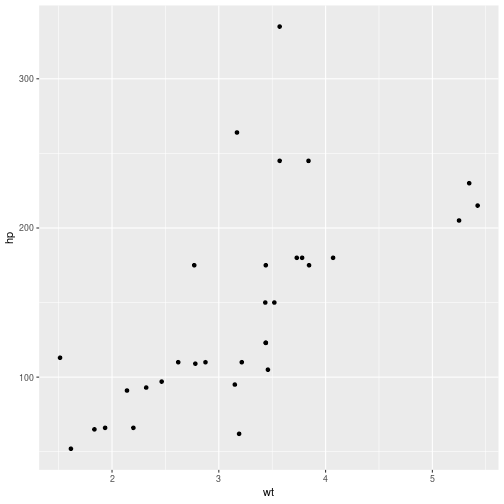
\includegraphics{figure/another-1.png}
\caption{plot of chunk another}
\end{figure}

Even more tesxt here.
\indent
\end{document}
